\documentclass[a4paper,12pt]{article}
\usepackage{polski}
\usepackage[utf8]{inputenc}
\usepackage[left = 3cm, right = 3cm, top = 2cm, bottom = 2cm]{geometry}
\usepackage{enumerate}
\usepackage{amssymb}		% pakiet do symboli
\usepackage{amsmath}		% pakiet do matmy
\usepackage{enumitem}		% punktowanie (a), (b), ...
\usepackage{nopageno}		% brak numerow stron
\usepackage{graphicx}		% wstawianie obrazkow
\usepackage{float}			% wstawianie obrazkow w dowolnym miejscu
\usepackage{titling}
%\usepackage[]{algorithm2e} 	% algorytmy :))
\usepackage{algpseudocode}	
%\usepackage{program}
%\usepackage{algorithmicx}
\usepackage{algorithm}

% nowe komendy dla wygodniejszego pisania :)
\newcommand{\subtitle}[1]{ \posttitle{ \par\end{center} \begin{center}\large#1\end{center} \vskip0.5em}}
\newcommand{\floor}[1]{\left\lfloor #1 \right\rfloor}
\newcommand{\ceil}[1]{\left\lceil #1 \right\rceil}
\newcommand{\code}[1]{\fontfamily{qcr}\selectfont\textbf{#1}\fontfamily{cmr}\selectfont}

\begin{document}
\noindent \textbf{Lista 4, zadanie 6.4 - Tomasz Woszczyński}\newline

\noindent \newline \textbf{Treść:} Ułóż algorytm, który dla danych podciągów $x$ i $y$ rozwiązuje problem znajdowania najdłuższego wspólnego podciągu niezawierającego podsłowa "egzamin". \newline

\noindent \textbf{Rozwiązanie:} Rozważmy najpierw problem znajdowania zbioru najdłuższych wspólnych podciągów $x[1...i]$ oraz $y[1...j]$. Wykorzystamy do tego dwie funkcje opisane poniżej, pod implementacją:\newline
\begin{algorithmic}
\Function{LCS}{$x$: string, $y$: string, $m$: $length(x)$, $n$: $length(y)$}
	\For{$i \gets 0$ to $m$}
		\For{$j \gets 0$ to $n$}
			\If{$i = 0$ or $j = 0$}
				\State $L[i][j] \gets 0$
			\ElsIf{$x[i-1] = y[j-1]$}
				\State $L[i][j] \gets L[i-1][j-1]+1$
			\Else
				\State $L[i][j] \gets \max(L[i-1][j], L[i][j-1])$
			\EndIf 
		\EndFor
	\EndFor
	\State \Return $L[m][n]$
\EndFunction
~\\
\Function{FindLCS}{$x$: string, $y$: string, $m$: $length(x)$, $n$: $length(y)$}
	\State $S \gets \emptyset$ \Comment{do tego zbioru będziemy zapisywać kolejne najdłuższe podciągi}
	\If{$i = 0$ or $j = 0$} \Comment{w tym miejscu dochodzimy do końca stringa}
		\State $S \cup \varepsilon$
		\State \Return $S$
	\EndIf
	\If{$x[m-1] = y[n-1]$} \Comment{ostatni znak $x$ i $y$ jest taki sam}
		\State $T \gets \Call{FindLCS}{$x, y, m - 1, n - 1$}$ \Comment{wywołujemy się rekurencyjnie}
		\ForAll{$str$ in $T$} \Comment{do wszystkich LCS dodajemy ostatni znak}
			\State $S \cup (str + x[m-1])$
		\EndFor
	\Else \Comment{ostatnie znaki podciągów $x$ i $y$ są różne}
		\If{$L[m-1][n] \geq L[m][n-1]$}\Comment{gdy LCS jest "od góry" w tablicy}
			\State $S \gets \Call{FindLCS}{$x, y, m - 1, n$}$\Comment{to idziemy do góry tablicy}
		\EndIf
		\If{$L[m][n-1] \geq L[m-1][n]$}\Comment{gdy LCS jest "od lewej" w tablicy}
			\State $T \gets \Call{FindLCS}{$x, y, m, n - 1$}$\Comment{to idziemy w lewą stronę tablicy}
			\ForAll{$str$ in $T$} \Comment{przechodzimy po wszystkich znalezionych LCS}
				\State $S \cup str$ \Comment{i dodajemy je do $S$}
			\EndFor
		\EndIf
	\EndIf
	\State \Return $S$ \Comment{otrzymujemy zbiór wszystkich najdłuższych podciągów $x$ i $y$}
\EndFunction
\end{algorithmic}

~\\ \noindent Funkcja LCS znajduje długość najdłuższego podciągu ciągów $x$ i $y$  w czasie $O(m\cdot n)$, gdzie $m$ i $n$ to długości tych ciągów. Po wywołaniu tej funkcji otrzymujemy tablicę $L[m][n]$, dzięki której możemy w łatwy sposób rekurencyjnie odtworzyć wszystkie możliwe do uzyskania najdłuższe podciągi $x$ i $y$ - zajmuje się tym funkcja FindLCS.

~\\ \noindent Załóżmy, że w szukanym podciągu nie chcemy napotkać słowa $k$, będącego w naszym przypadku słowem "egzamin". Mając zbiór $S$ wszystkich najdłuższych $s_i$ podciągów, możemy rozpatrzyć trzy możliwe scenariusze.
\begin{enumerate}
\item podsłowo $k$ jest na początku $s_i$,
\item podsłowo $k$ jest na końcu $s_i$,
\item podsłowo $k$ jest w środku $s_i$.
\end{enumerate}
\noindent Pierwsze dwie możliwości są trywialne, gdyż po przejrzeniu całego stringa $s_i$ wystarczy usunąć pierwszą lub ostatnią, w zależności od przypadku, literę, aby uzyskać najdłuższy podciąg bez podsłowa $k$. Wtedy w otrzymanym podciągu możemy znów natrafić na rozpatrzone już przypadki, lub na przypadek ostatni, który jest trochę bardziej złożony. Jeśli w trakcie przechodzenia przez $s_i$ napotkamy podsłowo, którego chcemy się pozbyć, zapamiętujemy indeks $l$ pierwszego znaku $k$ w $s_i$, dzięki czemu będziemy w łatwy sposób mogli operować na tym podciągu. Następnie musimy sprawdzić, który z możliwych podciągów będzie dłuższy: ten bez pierwszej litery $k$, czy ten bez ostatniej litery $k$.
\begin{figure}[H]
\centering
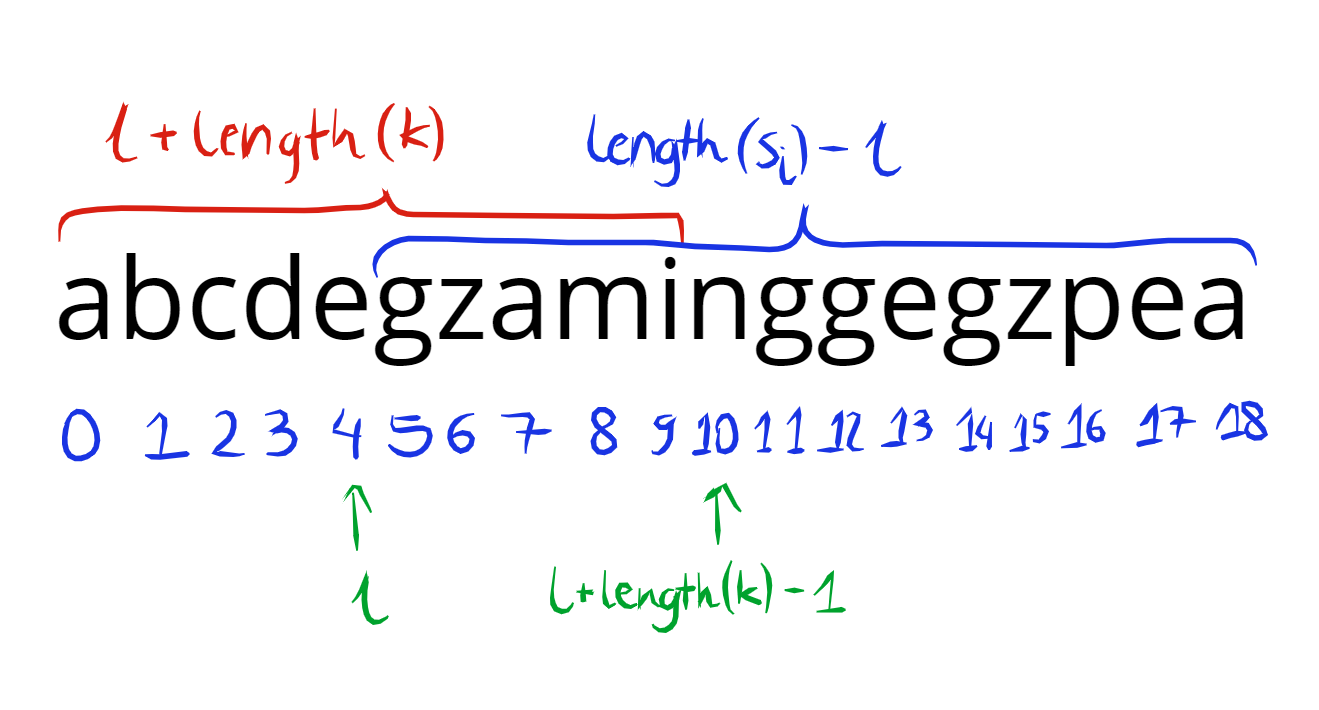
\includegraphics[width=1\textwidth]{lcs.png}
\end{figure}
\noindent Naszym zadaniem jest teraz porównanie wartości $l+\text{length}(k)$ z $\text{length}(s_i)-l$, wybieramy większą z nich i zapamiętujemy długość tego podciągu, jak i sam podciąg. W taki sposób musimy porównać wszystkie podciągi $s_i \in S$, a następnie wybrać najdłuższy z nich (gdy jest ich kilka, wybieramy dowolny). Złożoność czasowa algorytmu znajdowania najdłuższego podciągu z danego zbioru $S$ bez wybranego podsłowa $k$ wynosi $O(\vert S \vert \cdot \text{length}(s_1))$.

\end{document}